% This LaTeX document needs to be compiled with XeLaTeX.
\documentclass[10pt]{article}
\usepackage[utf8]{inputenc}
\usepackage{ucharclasses}
\usepackage{amsmath}
\usepackage{amsfonts}
\usepackage{amssymb}
\usepackage[version=4]{mhchem}
\usepackage{stmaryrd}
\usepackage{graphicx}
\usepackage[export]{adjustbox}
\graphicspath{ {./images/} }
\usepackage{multirow}
\usepackage[fallback]{xeCJK}
\usepackage{polyglossia}
\usepackage{fontspec}
\IfFontExistsTF{Noto Serif CJK SC}
{\setCJKmainfont{Noto Serif CJK SC}}
{\IfFontExistsTF{STSong}
  {\setCJKmainfont{STSong}}
  {\IfFontExistsTF{Droid Sans Fallback}
    {\setCJKmainfont{Droid Sans Fallback}}
    {\setCJKmainfont{SimSun}}
}}

\setmainlanguage{english}
\setotherlanguages{german}
\IfFontExistsTF{CMU Serif}
{\newfontfamily\lgcfont{CMU Serif}}
{\IfFontExistsTF{DejaVu Sans}
  {\newfontfamily\lgcfont{DejaVu Sans}}
  {\newfontfamily\lgcfont{Georgia}}
}
\setDefaultTransitions{\lgcfont}{}

\begin{document}
\section*{2020 AMC 8 Problems}
\section*{第1题}
Luka is making lemonade to sell at a school fundraiser.His recipe requires 4 times as much water as sugar and twice as much sugar as lemon juice.He uses 3 cups of lemon juice.How many cups of water does he need?

卢卡正在做柠檬水,准备在学校的募捐会上出售。他的配料表需要的水是糖的四倍,糖是柠檬汁的两倍。他用了 3 杯柠檬汁。他需要多少杯水?\\
(A) 6\\
(B) 8\\
(C) 12\\
(D) 18\\
(E) 24

\section*{第2题}
Four friends do yardwork for their neighbors over the weekend, earning $\$ 15, \$ 20, \$ 25$ ,and $\$ 40$ ,respectively.They decide to split their earnings equally among themselves.In total how much will the friend who earned $\$ 40$ give to the others?

四个朋友在周末为他们的邻居打扫院子,收入分别为 $\$ 15, \$ 20, \$ 25$ ,和 $\$ 40$ ,。他们决定平分收入。那么赚了 40 美元的那个朋友总共会给其他人多少钱?\\
(A)$\$ 5$\\
(B)$\$ 10$\\
(C)$\$ 15$\\
(D)$\$ 20$\\
(E)$\$ 25$

\section*{第3题}
Carrie has a rectangular garden that measures 6 feet by 8 feet.She plants the entire garden with strawberry plants.Carrie is able to plant 4 strawberry plants per square foot,and she harvests an average of 10 strawberries per plant.How many strawberries can she expect to harvest?

Carrie 有一个矩形的花园,尺寸是 6 英尺 $\times 8$ 英尺。她在整个花园里都种植了草莓。Carrie 每平方英尺种植 4 棵植株,并且每棵植株上她可以收获 10 颗草莓。那么她可以期望总共收获多少颗草莓?\\
(A) 560\\
(B) 960\\
(C) 1120\\
(D) 1920\\
(E) 3840

\section*{第4题}
Three hexagons of increasing size are shown below.Suppose the dot pattern continues so that each successive hexagon contains one more band of dots.How many dots are in the next hexagon?

三个面积逐渐增大的六边形如下图所示。假设这种点阵模式以此规律继续,使得后一个六边形比前一个多一层点带。那么图中下一个六边形中有多少个点?\\
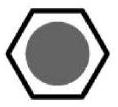
\includegraphics[max width=\textwidth, center]{2025_09_05_48544237b06df716137eg-02}\\
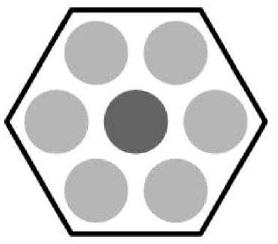
\includegraphics[max width=\textwidth, center]{2025_09_05_48544237b06df716137eg-02(2)}\\
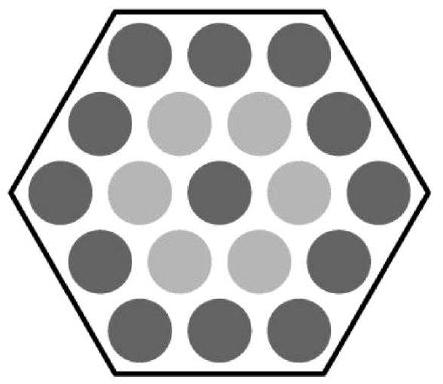
\includegraphics[max width=\textwidth, center]{2025_09_05_48544237b06df716137eg-02(1)}\\
(A) 35\\
(B) 37\\
(C) 39\\
(D) 43\\
(E) 49

\section*{第5题}
Three fourths of a pitcher is filled with pineapple juice.The pitcher is emptied by pouring an equal amount of juice into each of 5 cups.What percent of the total capacity of the pitcher did each cup receive?

一个水罐装了总容积四分之三的菠萝汁。然后把水罐里所有的菠萝汁平均倒到 5 个杯子里。那么每个杯子里菠萝汁的量占了水罐总容量的百分之几?\\
(A) 5\\
(B) 10\\
(C) 15\\
(D) 20\\
(E) 25

\section*{第6题}
Aaron,Darren,Karen,Maren,and Sharon rode on a small train that has five cars that seat one person each.Maren sat in the last car.Aaron sat directly behind Sharon.Darren sat in one of the cars in front of Aaron.At least one person sat between Karen and Darren.Who sat in the middle car?

Aaron,Darren,Karen,Maren,和 Sharon 乘坐一列小火车,火车有五节车厢,每节车厢可坐一人。Maren 坐在最后一节车厢里。Aaron 坐在 Sharon 的正后方。Darren 坐在亚伦前面的某节车厢里。至少有一个人坐在 Karen 和 Darren 之间。谁坐在中间的那节车厢里?\\
(A)Aaron\\
(B)Darren\\
(C)Karen\\
(D)Maren\\
(E)Sharon

\section*{第7题}
How many integers between 2020 and 2400 have four distinct digits arranged in increasing order?(For example, 2347 is one integer.) 2020 和 2400 之间有多少个整数,满足四个位上的数字都不相同,且按照升序排列?(例如, 2347 就是满足题意的一个数)\\
(A) 9\\
(B) 10\\
(C) 15\\
(D) 21\\
(E) 28

\section*{第8题}
Ricardo has 2020 coins,some of which are pennies( 1 -cent coins)and the rest of which are nickels(5-cent coins).He has at least one penny and at least one nickel.What is the difference in cents between the greatest possible and least possible amounts of money that Ricardo can have? Ricardo 有2020枚硬币,其中一些是便士(1 美分硬币),其余的是镍币(5 美分硬币)。他有至少一枚一分便士和一枚五分镍币。Ricardo可能拥有的最大金额和可能拥有的最小金额相差多少美分?\\
(A) 8062\\
(B) 8068\\
(C) 8072\\
(D) 8076\\
(E) 8082

\section*{第9题}
Akash's birthday cake is in the form of a $4 \times 4 \times 4$ inch cube.The cake has icing on the top and the four side faces,and no icing on the bottom. Suppose the cake is cut into 64 smaller cubes,each\\
measuring $1 \times 1 \times 1$ inch,as shown below.How many small pieces will have icing on exactly two sides?

Akash 的生日蛋糕是一个 $4 \times 4 \times 4$ 的正方体(边长单位:英寸)。这个立方体的顶部和 4 个侧面都有冰覆盖,但底面没有。假设这个正方体被分成 64 个 $1 \times 1 \times 1$ 英寸的小正方体,如下图所示。那么这些小正方体中有多少个恰好两面有冰?\\
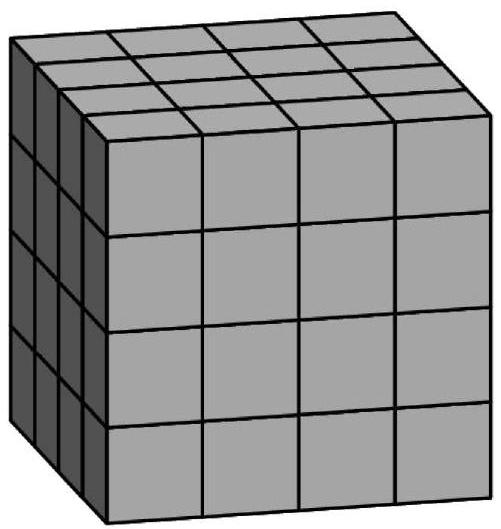
\includegraphics[max width=\textwidth, center]{2025_09_05_48544237b06df716137eg-05}\\
(A) 12\\
(B) 16\\
(C) 18\\
(D) 20\\
(E) 24

\section*{第10题}
Zara has a collection of 4 marbles:an Aggie,a Bumblebee,a Steelie,and a Tiger.She wants to display them in a row on a shelf,but does not want to put the Steelie and the Tiger next to one another.In how many ways can she do this?

Zara 有 4 个玻璃球,分别叫 Aggie,Bumblebee,Steelie,和 Tiger。她想把它们在架子上排成一行,但不想让 Steelie 和 Tiger 相邻。那么她有多少种排列方法?\\
(A) 6\\
(B) 8\\
(C) 12\\
(D) 18\\
(E) 24

\section*{第11题}
After school,Maya and Naomi headed to the beach, 6 miles away.Maya decided to bike while Naomi took a bus.The graph below shows their journeys,indicating the time and distance traveled.What was the difference,in miles per hour,between Naomi's and Maya's average speeds?

放学后,Maya 和 Naomi 出发去距学校 6 英里的沙滩。Maya 决定骑车去,而 Naomi 坐公交车去。下图展示了他们的行程,显示了时间和所走路程的关系。那么 Naomi 和 Maya 的平均速度之差是多少英里每小时?\\
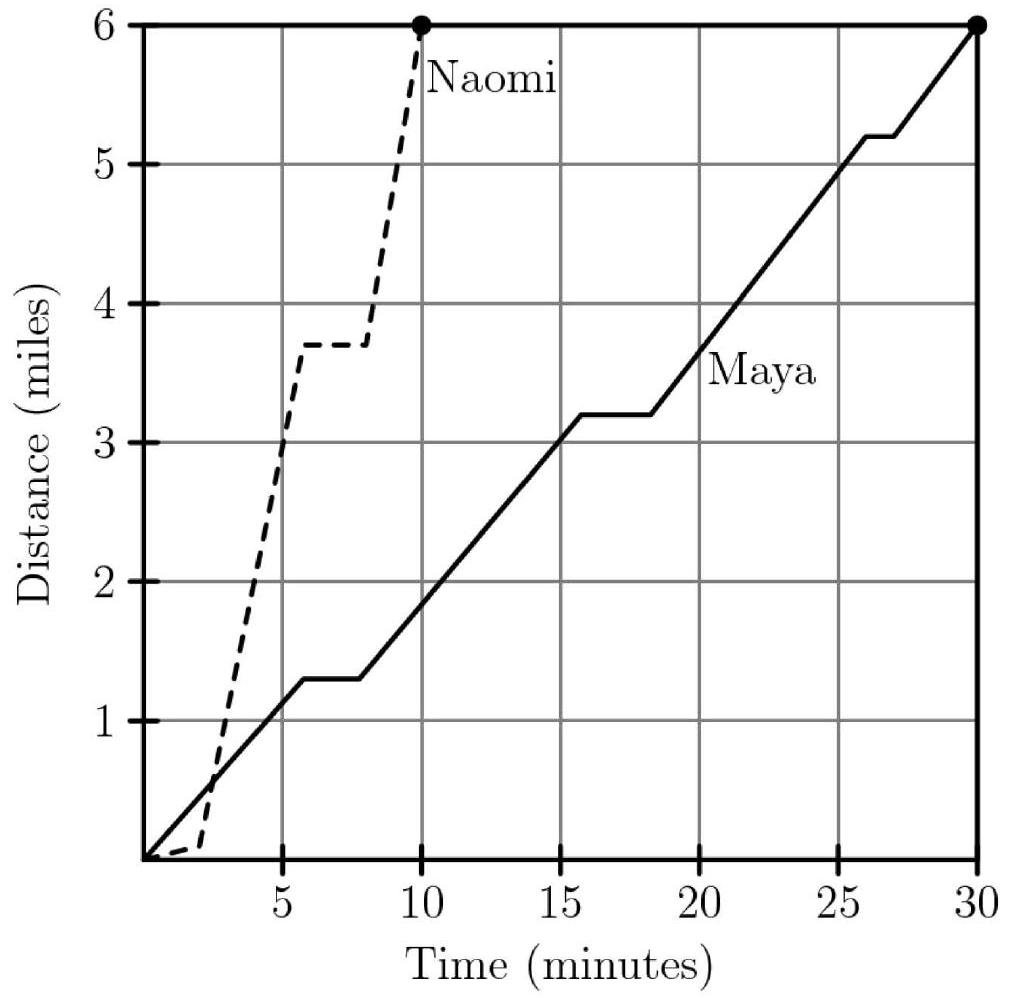
\includegraphics[max width=\textwidth, center]{2025_09_05_48544237b06df716137eg-06}\\
(A) 6\\
(B) 12\\
(C) 18\\
(D) 20\\
(E) 24

\section*{第12题}
For a positive integer $n$ ,the factorial notation $n$ !represents the product of the integers from $n$ to 1 .(For example, $6!=6 \cdot 5 \cdot 4 \cdot 3 \cdot 2 \cdot 1$ .)What value of $N$ satisfies the following equation?

$$
5!\cdot 9!=12 \cdot N!
$$

对一个正整数 $n$ ,符号 $n!$ 表示从 $n$ 到 1 的所有整数的乘积。(例如, $6!=6 \cdot 5 \cdot 4 \cdot 3 \cdot 2 \cdot 1$ )则 $N$ 为何值时,满足下面的方程?

$$
5!\cdot 9!=12 \cdot N!
$$

(A) 10\\
(B) 11\\
(C) 12\\
(D) 13\\
(E) 14

\section*{第13题}
Jamal has a drawer containing 6 green socks, 18 purple socks, and 12 orange socks.After adding more purple socks,Jamal noticed that there is now a 60\textbackslash %chance that a sock randomly selected from the drawer is purple.How many purple socks did Jamal add? Jamal 有个抽屉,内有 6 只绿色袜子, 18 只紫色袜子, 12 只橙色袜子。当加了更多紫色袜子后,Jamal 发现,从抽屉里随机抽取一只袜子,有 $60 \%$ 的概率它是紫色的。那么 Jamal 加了多少只紫袜子?\\
(A) 6\\
(B) 9\\
(C) 12\\
(D) 18\\
(E) 24

\section*{第14题}
There are 20 cities in the County of Newton.Their populations are shown in the bar chart below.The average population of all the cities is indicated by the horizontal dashed line.Which of the following is closest to the total population of all 20 cities?

牛顿县有 20 座城市。下面的条形图显示了各个城市的人口数。所有城市的平均人口数用一条水平虚线表示。以下哪一项最接近这 20 座城市的总人口?\\
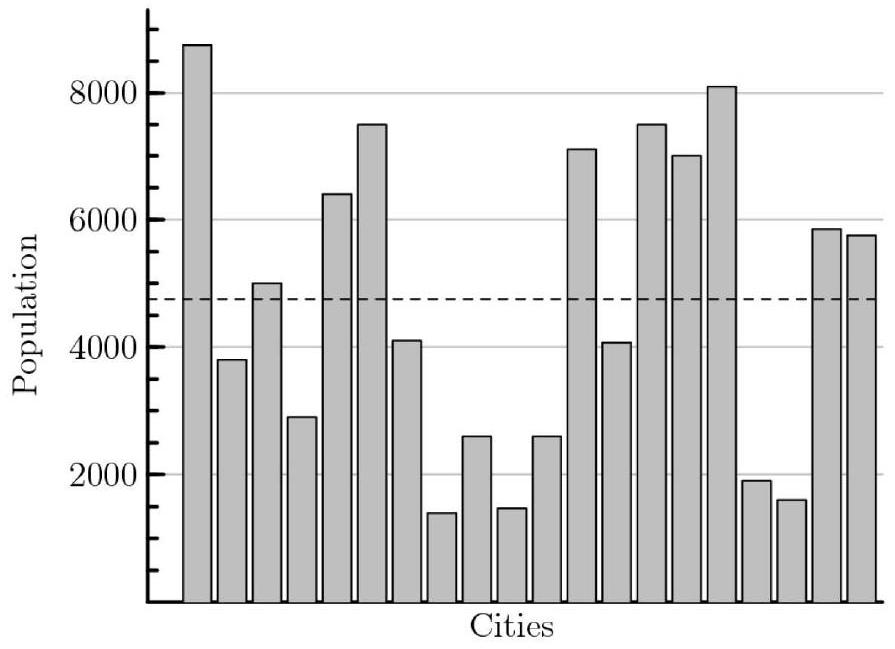
\includegraphics[max width=\textwidth, center]{2025_09_05_48544237b06df716137eg-08}\\
(A) 65,000\\
(B) 75,000\\
(C) 85,000\\
(D) 95,000\\
(E) 105,000

\section*{第15题}
Suppose $15 \%$ of $x$ equals $20 \%$ of $y$ .What percentage of $x$ is $y$ ?\\
假设 $x$ 的 $15 \%$ 等于 $y$ 的 $20 \%$ 。那么 $x$ 的百分之几是 $y$ ?\\
(A) 5\\
(B) 35\\
(C) 75\\
(D) $133 \frac{1}{3}$\\
(E) 300

\section*{第16题}
Each of the points $A, B, C, D, E$ ,and $F$ in the figure below represents a different digit from 1 to 6 .Each of the five lines shown passes through some of these points.The digits along each line are added to produce five sums,one for each line.The total of the five sums is 47 .What is the digit represented by B?

下图中 $A, B, C, D, E$ ,和 $F$ 中的每个点代表1到 6 之间的一个不同的数字.图中所示的 5 条直线,每条都会通过其中几个点。每条直线上的几个数字相加得到 5 个和,每条直线一个和。把这 5 个和相加,结果为 47 。那么 B 代表的数字是多少?\\
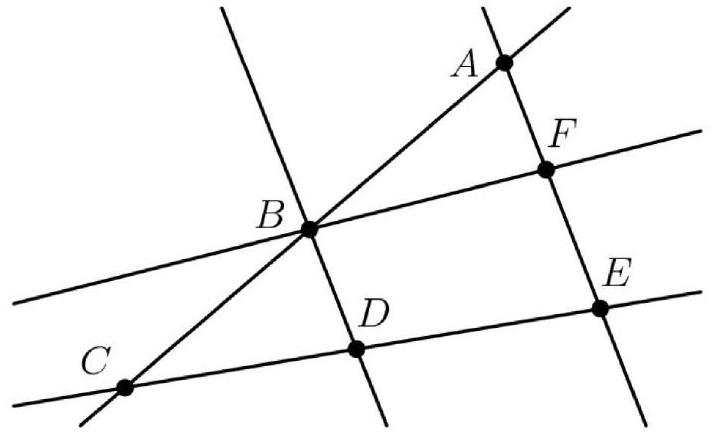
\includegraphics[max width=\textwidth, center]{2025_09_05_48544237b06df716137eg-09}\\
(A) 1\\
(B) 2\\
(C) 3\\
(D) 4\\
(E) 5

\section*{第17题}
How many factors of 2020 have more than 3 factors?(As an example, 12 has 6 factors,namely $1,2,3,4,6$ ,and 12 .)

2020 有多少个因子,它们各自的因子个数都大于 3 ?(例如, 12 有 6 个因子,即, $1,2,3,4,6$ ,和12.)\\
(A) 6\\
(B) 7\\
(C) 8\\
(D) 9\\
(E) 10

\section*{第18题}
Rectangle $A B C D$ is inscribed in a semicircle with diameter $\overline{F E}$ ,as shown in the figure.Let $D A=16$ ,and let $F D=A E=9$ .What is the area of $A B C D$ ?

矩形 ABCD 内接在直径为 $\overline{F E}$ 的半圆中,如图所示。已知\\
$D A=16, F D=A E=9$ .则 ABCD 的面积是多少?\\
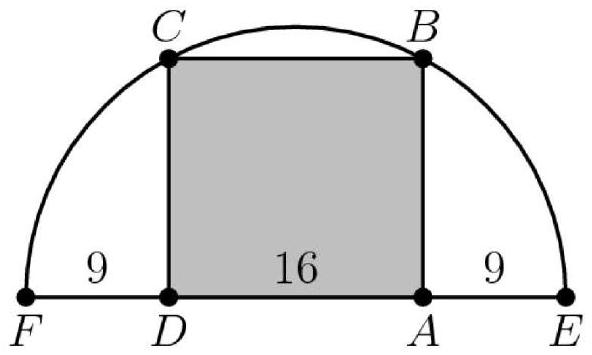
\includegraphics[max width=\textwidth, center]{2025_09_05_48544237b06df716137eg-10}\\
(A) 240\\
(B) 248\\
(C) 256\\
(D) 264\\
(E) 272

\section*{第19题}
A number is called flippy if its digits alternate between two distinct digits. For example, 2020 and 37373 are flippy,but 3883 and 123123 are not. How many five-digit flippy numbers are divisible by 15 ?若一个数的各个位上数字在 2 个不同的数字之间交替出现,那么这个数称为 flippy.例如, 2020 和 37373 都是 flippy 数,但是 3883 和 123123 不是。有多少个 5 位 flippy 数能被 15 整除?\\
(A) 3\\
(B) 4\\
(C) 5\\
(D) 6\\
(E) 8

\section*{第20题}
A scientist walking through a forest recorded as integers the heights of 5 trees standing in a row.She observed that each tree was either twice as tall or half as tall as the one to its right.Unfortunately some of her data was lost when rain fell on her notebook.Her notes are shown below,with blanks indicating the missing numbers.Based on her observations,the scientist was able to reconstruct the lost data.What was the average height of the trees,in meters?

一个穿过森林的科学家将一排 5 棵树的高度都记录了下来,这 5 棵树的高度均为整数。她观察到,每棵树的高度要么是右边树高的 2 倍,要么是它的一半。不幸的是,由于雨水落在她的笔记本上,导致部分数据丢失。她的笔记如下图所示,空白部分表示丢失的数据。根据她的观察,这个科学家最终能够重建丢失的数据。那么这 5 棵树的平均高度是多少米?

\begin{center}
\begin{tabular}{|c|c|}
\hline
Tree 1 & — meters \\
Tree 2 & 11 meters \\
Tree 3 & — meters \\
Tree 4 & — meters \\
Tree 5 & — meters \\
\hline
Average height & — .2 meters \\
\hline
\end{tabular}
\end{center}

(A) 22.2\\
(B) 24.2\\
(C) 33.2\\
(D) 35.2\\
(E) 37.2

\section*{第21题}
A game board consists of 64 squares that alternate in color between black and white.The figure below shows square $P$ in the bottom row and square $Q$ in the top row.A marker is placed at $P$ .A step consists of moving the marker onto one of the adjoining white squares in the row above.How many 7 -step paths are there from $P$ to $Q$ ?(The figure shows a sample path.)

一种游戏板由 64 个黑白相间的方块组成。下图显示了底行中的一个正方形 P 和顶行中的一个正方形 Q 。在正方形 P 上放了一个标记,将标记移到上面一行中相邻的一个白色正方形上,这个操作称为一步。从 P 到 Q 有多少种 7 步路径?(图中显示了一种可能的示例路径)。\\
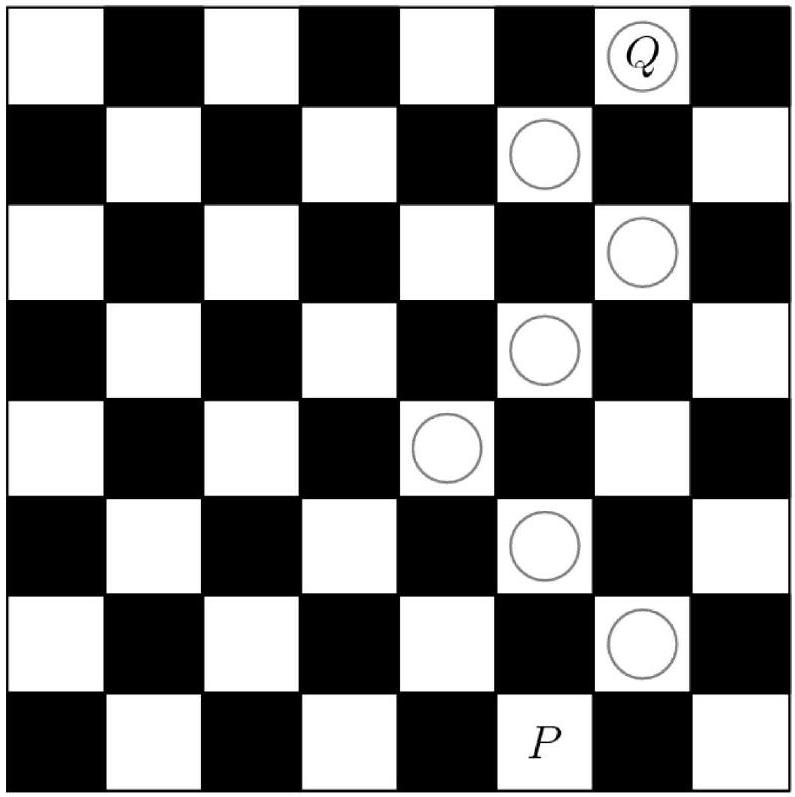
\includegraphics[max width=\textwidth, center]{2025_09_05_48544237b06df716137eg-12}\\
(A) 28\\
(B) 30\\
(C) 32\\
(D) 33\\
(E) 35

\section*{第22题}
When a positive integer $N$ is fed into a machine,the output is a number calculated according to the rule shown below.\\
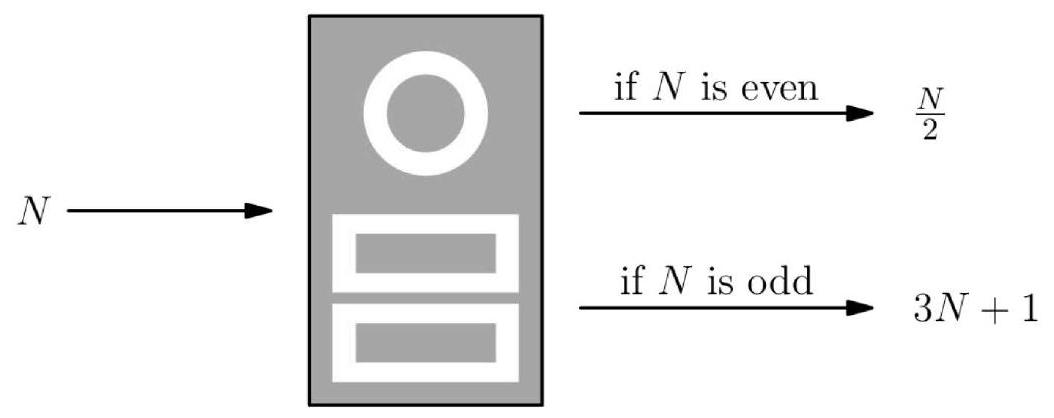
\includegraphics[max width=\textwidth, center]{2025_09_05_48544237b06df716137eg-13}

For example,starting with an input of $N=7$ ,the machine will output $3 \cdot 7+1=22$ .Then if the output is repeatedly inserted into the machine five more times,the final output is

$$
26.7 \rightarrow 22 \rightarrow 11 \rightarrow 34 \rightarrow 17 \rightarrow 52 \rightarrow 26
$$

When the same 6 -step process is applied to a different starting value of $N$ ,the final output is 1 .What is the sum of all such integers $N$ ?

$$
N \rightarrow \_\rightarrow \_\rightarrow \_\rightarrow \_\rightarrow \_\rightarrow 1
$$

当把一个正整数 N 输入一个机器,输出的是一个根据下面规则计算得到的数字:\\
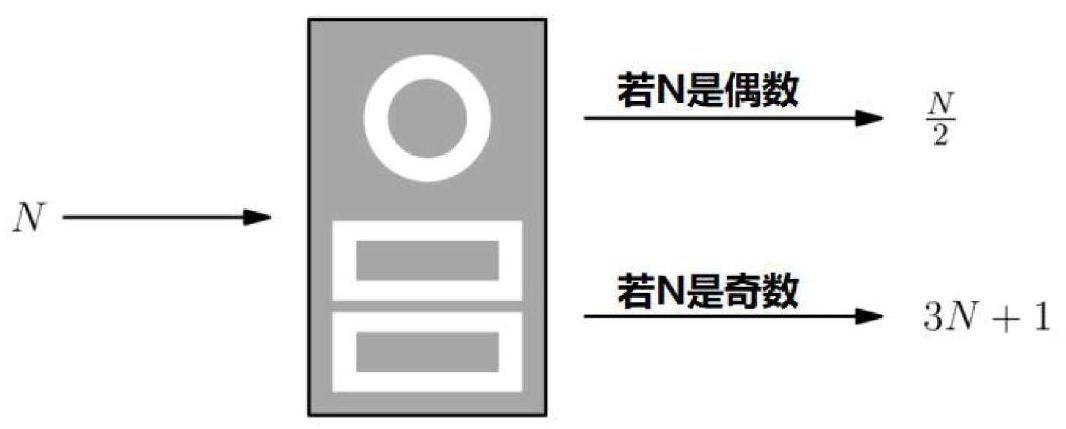
\includegraphics[max width=\textwidth, center]{2025_09_05_48544237b06df716137eg-13(1)}

例如,一开始输入是 $N=7$ ,那么机器将输出 $3 \cdot 7+1=22$ .然后如果把输出再输入机器这样继续重复 5 次,那么最后的输出将是

$$
7 \rightarrow 22 \rightarrow 11 \rightarrow 34 \rightarrow 17 \rightarrow 52 \rightarrow 26
$$

当把上述同样的 6 步过程再作用于另一个不同的初始值 N ,最终的输出是1.那么 N 的所有可能值之和是多少?

$$
N \rightarrow \_\rightarrow \_\rightarrow \_\rightarrow \_\rightarrow \_\rightarrow 1
$$

(A) 73\\
(B) 74\\
(C) 75\\
(D) 82\\
(E) 83

\section*{第23题}
Five different awards are to be given to three students.Each student will receive at least one award.In how many different ways can the awards be distributed?

把 5 个不同的奖章分配给 3 个学生,每个学生得到至少一个奖章。那么一共有多少种不同的分配方法?\\
(A) 120\\
(B) 150\\
(C) 180\\
(D) 210\\
(E) 240

\section*{第24题}
A large square region is paved with $n^{2}$ gray square tiles,each measuring $s$ inches on a side.A border $d$ inches wide surrounds each tile. The figure below shows the case for $n=3$ .When $n=24$ ,the 576 gray tiles cover $64 \%$ of the area of the large square region.What is the ratio $\frac{d}{s}$ for this larger value of $n$ ?

一个大的正方形区域是用 $n^{2}$ 个灰色的方形瓷砖铺成的,每块的边长都是 $s$ 英寸。每一块瓷砖周围都有一个 $d$ 英寸宽的边框。下图显示了 $n=3$的情况。当 $n=24,576$ 块灰色瓷砖覆盖了大正方形面积的 $64 \%$ 。对于这个较大的 n 值,$\frac{d}{s}$ 的比值是多少?\\
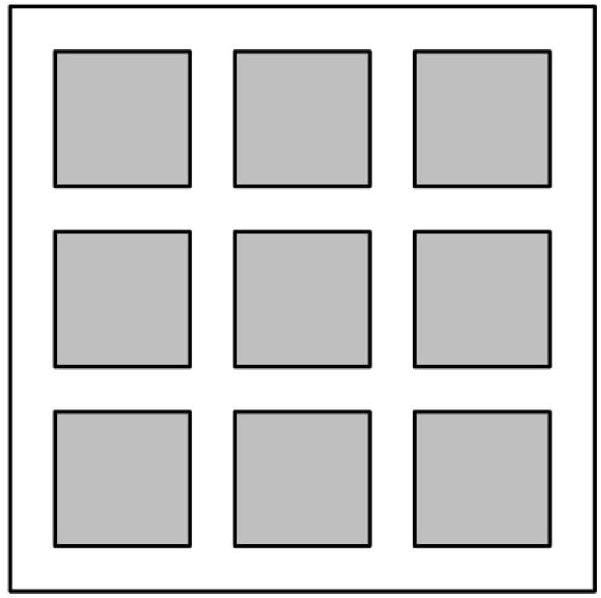
\includegraphics[max width=\textwidth, center]{2025_09_05_48544237b06df716137eg-15}\\
(A)$\frac{6}{25}$\\
(B)$\frac{1}{4}$\\
(C)$\frac{9}{25}$\\
(D)$\frac{7}{16}$\\
(E)$\frac{9}{16}$

\section*{第25题}
Rectangles $R_{1}$ and $R_{2}$ ,and squares $S_{1}, S_{2}$ ,and $S_{3}$ ,shown below,combine to form a rectangle that is 3322 units wide and 2020 units high.What is the side length of $S_{2}$ in units?

矩形 $R_{1}$ 和 $R_{2}$ ,正方形 $S_{1}, S_{2}$ ,和 $S_{3}$ ,如下图所示,拼成了一个宽为 3322 ,高为 2020 的大矩形。求 $S_{2}$ 的边长是多少?

\begin{center}
\begin{tabular}{|c|c|c|}
\hline
\multirow{2}{*}{$S_{1}$} & \multicolumn{2}{|c|}{$R_{2}$} \\
\cline { 2 - 2 }
 & $S_{2}$ &  \\
\cline { 1 - 1 }
\multicolumn{2}{|c|}{$S_{3}$} &  \\
\hline
\multicolumn{2}{|c|}{$R_{1}$} &  \\
\hline
\end{tabular}
\end{center}

(A) 651\\
(B) 655\\
(C) 656\\
(D) 662\\
(E) 666


\end{document}